% Executive Summary — separate deliverable (max 1,000 words per handbook).
% Standalone document; compile with pdflatex executive_summary.tex
\documentclass[10pt,twocolumn]{article}
\usepackage[margin=2.0cm,columnsep=0.8cm]{geometry}
\usepackage[T1]{fontenc}
\usepackage[utf8]{inputenc}
\usepackage{lmodern}
\usepackage{microtype}
\usepackage{graphicx}
\usepackage{amsmath}
\usepackage{float}
\usepackage[font=footnotesize,labelfont=bf]{caption}
\usepackage{titlesec}
\titleformat{\section}{\normalsize\bfseries}{}{0pt}{}
\titlespacing{\section}{0pt}{0.9em}{0.35em}

\title{\large\bfseries HYBRID FOURIER NEURAL OPERATORS FOR TIME-DOMAIN
BLACK-HOLE PERTURBATIONS AND QUASINORMAL MODE EXTRACTION\\[0.3em]
\normalfont\normalsize\scshape Executive Summary}
\author{\small Jonathan Chung \quad$|$\quad MPhil Data Intensive Science
\quad$|$\quad University of Cambridge}
\date{}

\begin{document}
\maketitle

\section{Motivation \& Scientific Justification}

A perturbed black hole settles by emitting a ringdown signal composed
of damped oscillations, the quasinormal modes (QNMs). For each mode of
a Kerr black hole, general relativity fixes the frequency and damping
time through the remnant mass and spin [1,2]. Measuring these tones in
gravitational-wave data tests whether the remnant is consistent with
the Kerr prediction, an observational programme opened by the
ringdown analysis of GW150914 [3]. Reliable spectroscopy requires an
accurate time-domain waveform and a fit interval in which the QNM
model is valid [4].

Physics-informed neural networks (PINNs) approximate differential
equations by minimising their governing-equation, initial-data and
boundary residuals. Patel et al. [5] solve the Regge--Wheeler and
Zerilli equations in the time domain, but report relative $L^2$ field
errors of $23.59\%$ and $28.06\%$, respectively, and select one fit
window manually. We first reproduce and improve this calculation. We
then introduce a Schwarzschild hybrid Fourier neural operator (hFNO)
that corrects a reduced-resolution numerical prior across mass and
initial-data parameters. A single trained hFNO predicts fields for new
configurations without per-configuration neural-network retraining.

\section{Methodology}

The reproduction uses Patel et al.'s network architecture, loss
weights and optimiser schedule. An enhanced PINN then doubles the
L-BFGS optimisation budget and adds residual-greedy sampling, placing
more training points where the equation residual is largest.

For the Schwarzschild hFNO, Richardson extrapolation of the $k=2$ and
$k=4$ coarse fields produces a field estimate whose difference from
the deployment prior defines the correction target [6]. At inference,
the reconstruction is
\begin{equation}
	\Phi^{\mathrm{hyb}}(x,t)
	= \mathcal U\Phi^{\mathrm c}(x,t)
	+ g(x,t)\,\mathcal H_\theta(X)(x,t).
	\label{eq:es-hfno}
\end{equation}
Here $\mathcal U$ denotes quintic upsampling, $\Phi^{\mathrm c}$ the
deployed $k=4$ coarse field, $\mathcal H_\theta$ the four-layer FNO
correction operator [7--9], and $g$ the deterministic fixed-scale
gradient gate derived from the numerical prior. The fine FD reference
field is used only for evaluation and does not enter the training
loss. Coarsening both space and time by four reduces the
finite-difference point-update count to approximately one-sixteenth of
the fine-grid evolution. Each new configuration requires one $k=4$
evolution, quintic upsampling and one neural-operator evaluation.

An independently trained Kerr hFNO corrects the complex spin-$-2$
Teukolsky field evolved on a horizon-penetrating hyperboloidal domain
[10,11]. Its correction target is constructed from independently
evolved $N=201$ and $N=401$ fourth-order fields; the $N=801$ fine
reference field is used only for evaluation. Unlike the Schwarzschild
model, the Kerr correction is ungated because a gradient gate would
suppress corrections in the low-amplitude ringdown at future null
infinity. QNMs are extracted from the Schwarzschild observer waveform
at $x_q=10M$ and the Kerr waveform at future null infinity. For
Schwarzschild, fit-window scans identify stable contiguous blocks of
frequency and damping-time estimates. For Kerr, real-component and
complex-field estimators generate candidate poles, and the
spin-dependent Leaver pole identifies the labelled $(4,2,0)$ mode
without replacing the fitted values.

\section{Key Findings}

\begin{figure}[H]
\centering
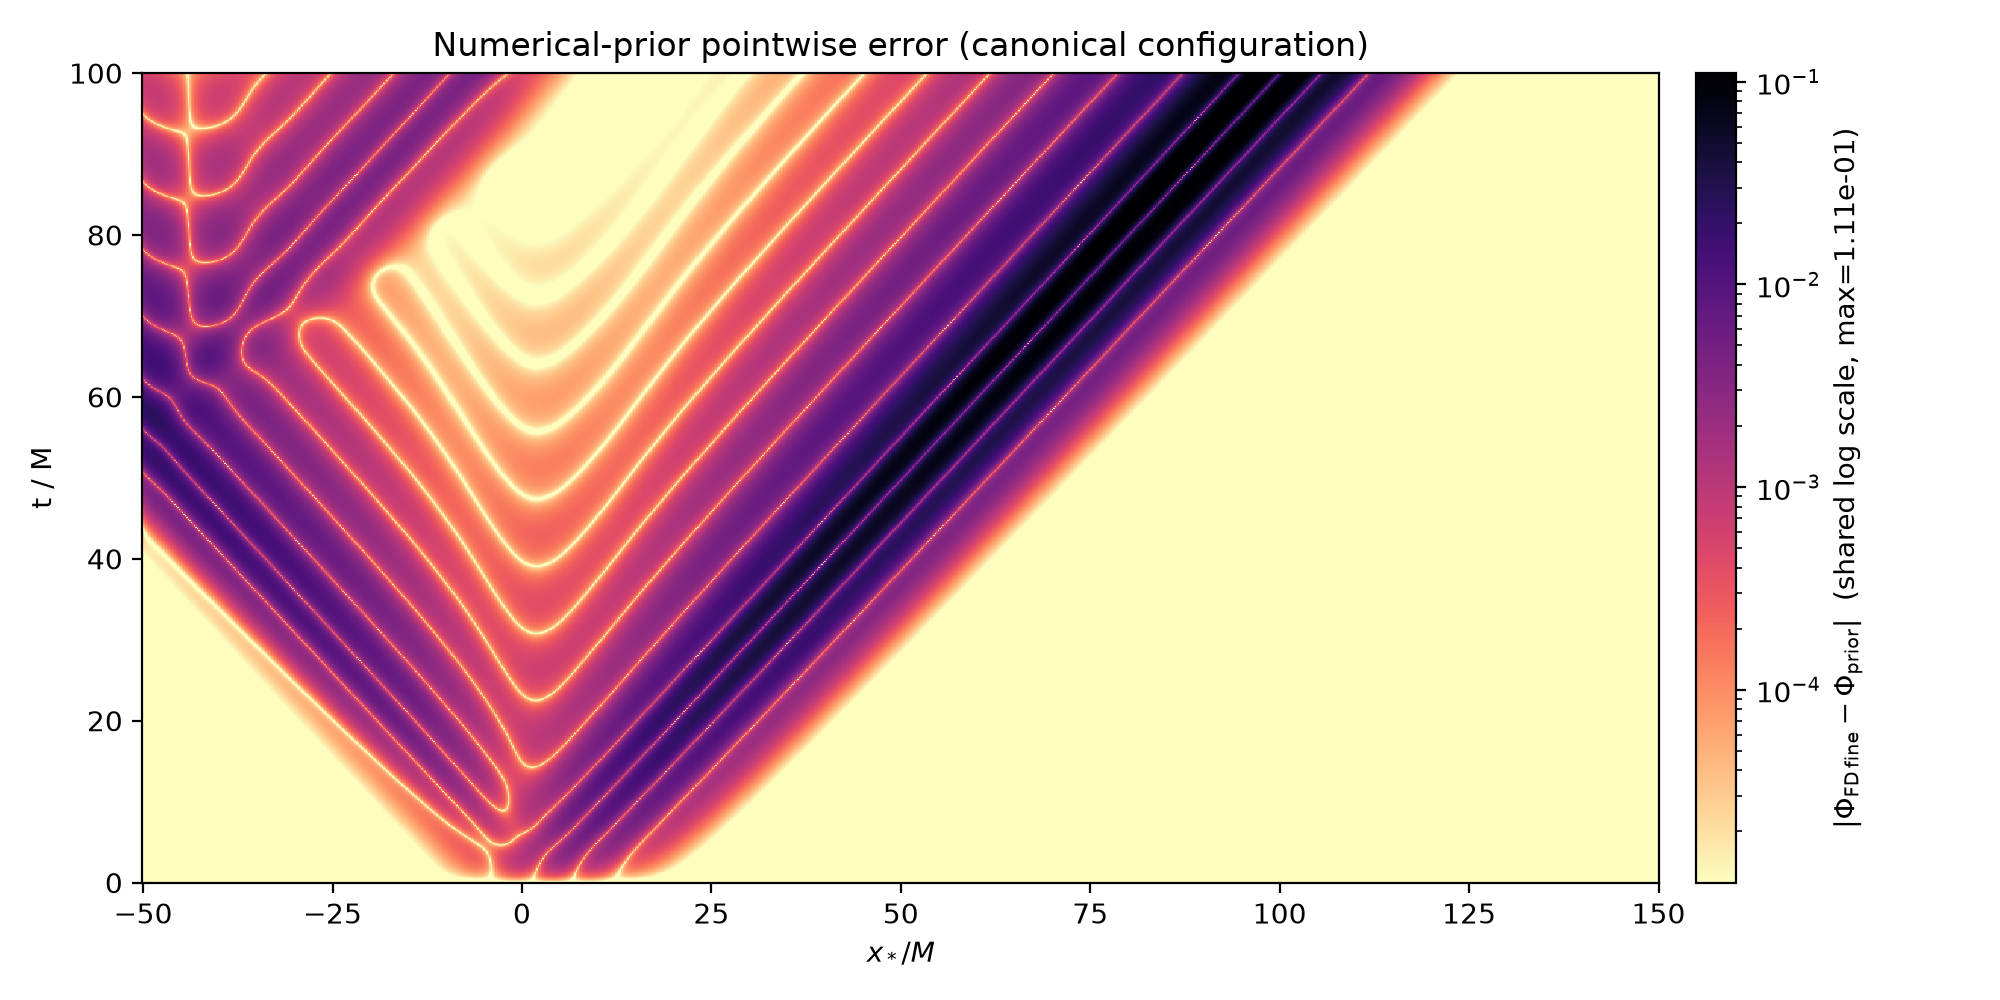
\includegraphics[width=0.78\columnwidth]{../outputs/hybrid/fno_sw_gate_s1em3_t100/figs/hybrid_pointwise_error_baseline.png}\\[-0.2em]
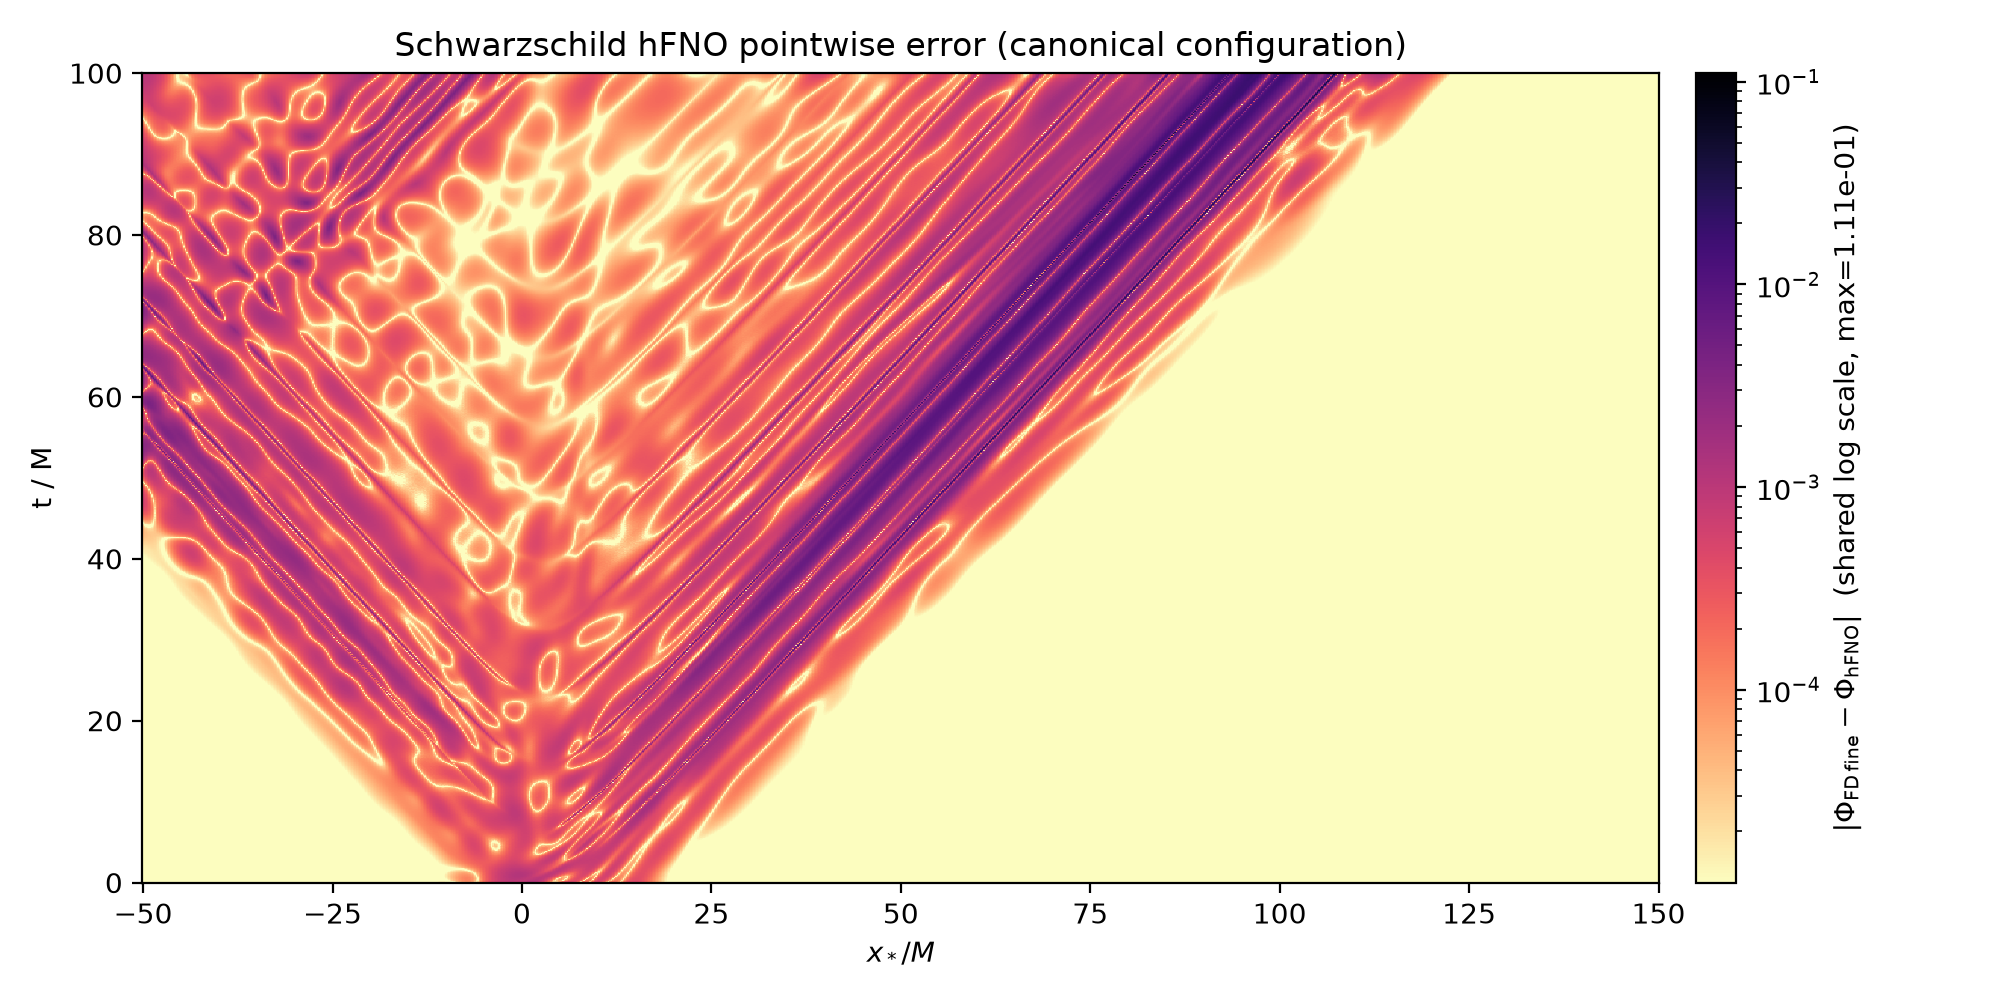
\includegraphics[width=0.78\columnwidth]{../outputs/hybrid/fno_sw_gate_s1em3_t100/figs/hybrid_pointwise_error.png}
\caption{Pointwise Schwarzschild field error on the canonical
configuration for the numerical prior (top) and hFNO (bottom), shown
on the same logarithmic scale. The hFNO substantially reduces the
coherent numerical-prior error bands, while structured wavefront and
late-time errors remain.}
\label{fig:es-error-maps}
\end{figure}

Our reproduction obtains relative $L^2$ field errors of $2.61\%$ for
Zerilli and $2.67\%$ for Regge--Wheeler, compared with the published
$28.06\%$ and $23.59\%$. The enhanced PINN reaches $0.58\%$ relative
$L^2$ field error. From its observer waveform, the M4 two-mode
fit-window plateau estimate gives a $0.029\%$ fundamental-frequency
error, while the M2 single-mode nonlinear least-squares fit gives a
$1.99\%$ damping-time error relative to Leaver's continued-fraction
values [12].

Across $100$ independent Schwarzschild configurations, the hFNO
reduces the mean relative $L^2$ error from $13.39\%$ for the numerical
prior to $1.85\%$, and the mean-squared field error by a factor of
$46$. M4 gives a median fundamental QNM frequency error of $0.152\%$.
Figure~1 shows that the hFNO substantially reduces the coherent
wavefront-error bands of the numerical prior, while structured
wavefront and late-time errors remain.

Across $128$ independent Kerr configurations spanning
$a/M\in[0,0.95]$, the independently trained hFNO reduces the median
relative $L^2$ error from $59.5\%$ for the numerical prior to
$0.78\%$. Under retrospective Leaver-closest reporting, the candidate
estimate with the smallest Leaver error is selected separately for
frequency and damping time after extraction. The resulting median
errors are $0.33\%$ in frequency and $1.52\%$ in damping time,
compared with $0.05\%$ and $0.27\%$ for the fine reference field.
Complete per-estimator results show substantial method dependence.

\begin{figure}[H]
\centering
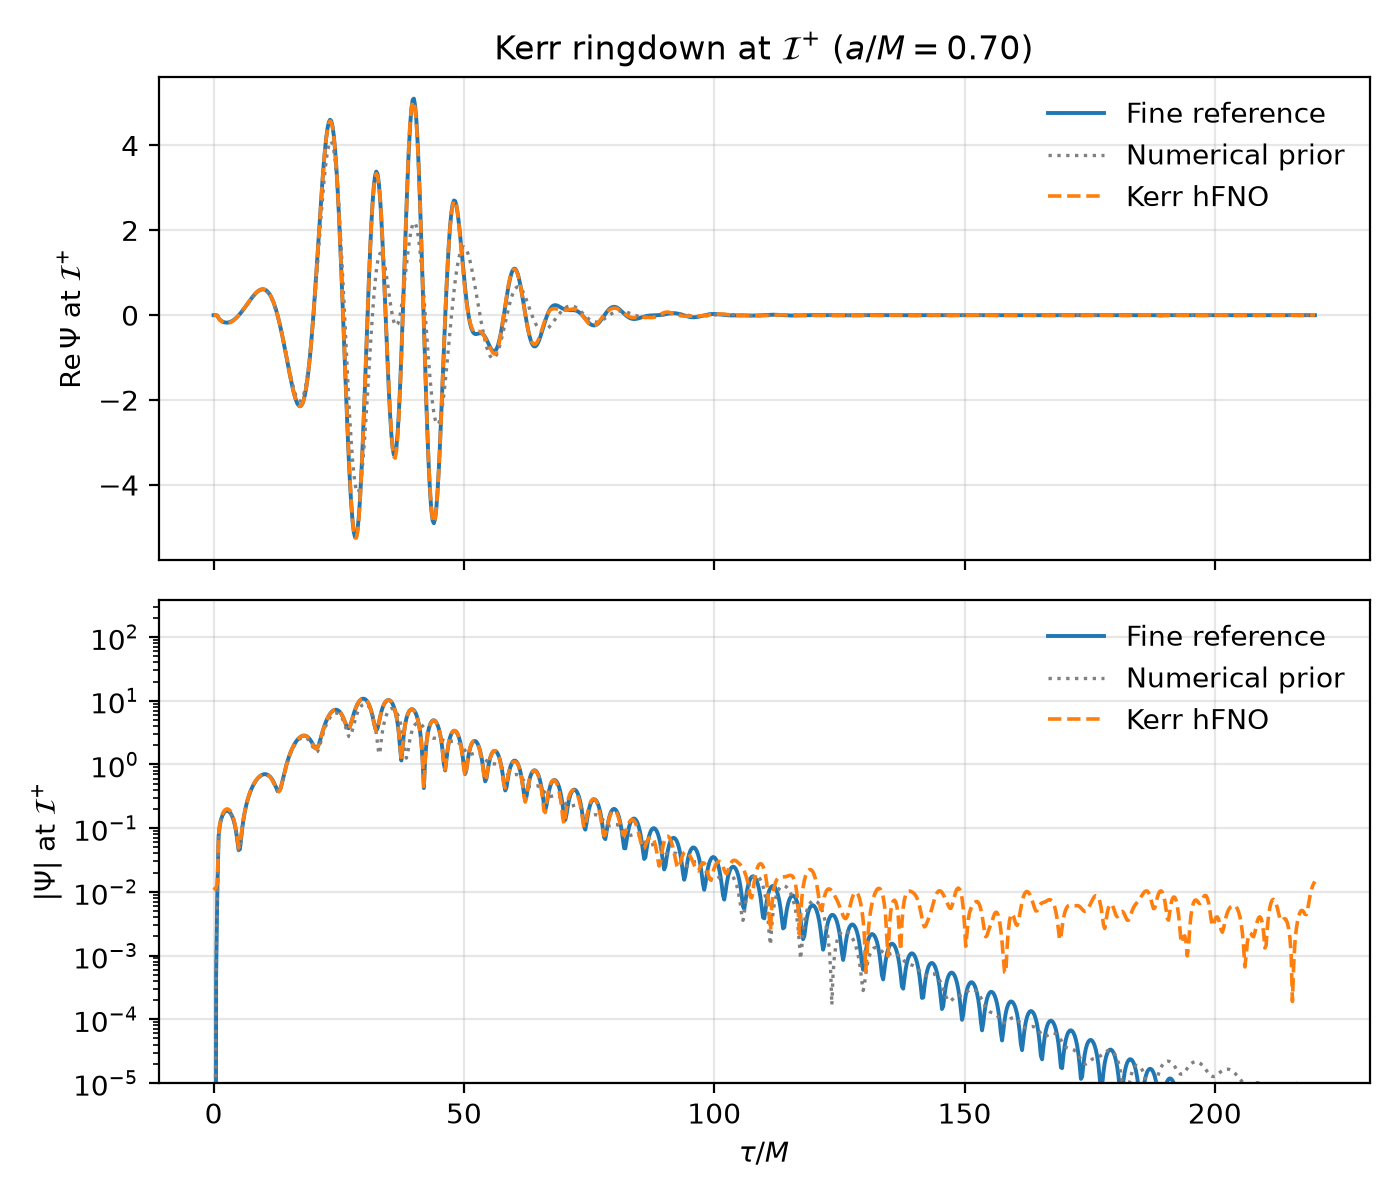
\includegraphics[width=0.96\columnwidth]{../outputs/kerr/figs/hybrid_ringdown_scri.png}
\caption{Kerr ringdown at future null infinity for a test
configuration nearest $a/M=0.70$. The Kerr hFNO follows the fine
reference through the prompt response and early ringdown, whereas the
numerical prior is visibly under-resolved. The logarithmic panel
reveals the hFNO's late-time residual, which limits damping-time
recovery.}
\label{fig:es-kerr-ringdown}
\end{figure}

\section{Recommendation \& Next Steps}

The first priority is a late-time-sensitive training objective that
improves the low-amplitude Kerr ringdown. Further tests should cover
additional harmonics and initial data, parameters outside the training
ranges, and changes of numerical domain and resolution. End-to-end
timing should quantify the wall-clock reduction and training
break-even point, including numerical evolution, interpolation and
neural inference. The resulting waveform families can then be
combined with reduced-order likelihood methods to test their practical
value for Bayesian parameter estimation [13].

\section{Research Impact \& Conclusion}

The separately trained Schwarzschild and Kerr hFNOs each combine a
reduced-resolution numerical prior with a correction learned across
their respective parameter family. The numerical prior supplies
characteristic propagation, potential scattering and boundary
treatment, while the neural operator predicts a discretisation-error
correction. Neither hFNO uses fine-grid reference fields in its
training loss, and neither requires per-configuration neural-network
retraining. The Schwarzschild M4 analysis and retrospective Kerr
analysis both give sub-percent median fundamental-frequency errors
while reducing the required numerical evolution. The hFNOs support
repeated field generation across the tested families and can be
assessed directly in future gravitational-wave likelihood
calculations. The coexistence of $0.78\%$ median global Kerr field
error and $1.52\%$ damping-time error is consistent with gridwise MSE
giving little weight to the low-amplitude late-time ringdown.

\begin{thebibliography}{13}
\scriptsize
\setlength{\itemsep}{0pt}
\setlength{\parskip}{0pt}
\bibitem{v70} C. V. Vishveshwara, \emph{Nature} \textbf{227},
936--938 (1970).
\bibitem{berti09} E. Berti, V. Cardoso, and A. O. Starinets,
\emph{Class. Quantum Grav.} \textbf{26}, 163001 (2009).
\bibitem{ligo16} LIGO Scientific Collaboration and Virgo
Collaboration, \emph{Phys. Rev. Lett.} \textbf{116}, 221101 (2016).
\bibitem{isi21} M. Isi and W. M. Farr, arXiv:2107.05609 [gr-qc]
(2021).
\bibitem{patel24} N. Patel, A. Aykutalp, and P. Laguna,
arXiv:2401.01440 [gr-qc] (2024).
\bibitem{richardson11} L. F. Richardson, \emph{Phil. Trans. R. Soc.
A} \textbf{210}, 307--357 (1911).
\bibitem{li21} Z. Li \emph{et al.}, International Conference on
Learning Representations (2021).
\bibitem{um20} K. Um \emph{et al.}, \emph{Adv. Neural Inf. Process.
Syst.} \textbf{33}, 6111--6122 (2020).
\bibitem{kochkov21} D. Kochkov \emph{et al.}, \emph{Proc. Natl.
Acad. Sci. USA} \textbf{118}, e2101784118 (2021).
\bibitem{teukolsky73} S. A. Teukolsky, \emph{Astrophys. J.}
\textbf{185}, 635--648 (1973).
\bibitem{harms13} E. Harms, S. Bernuzzi, and B. Br\"ugmann,
\emph{Class. Quantum Grav.} \textbf{30}, 115013 (2013).
\bibitem{leaver85} E. W. Leaver, \emph{Proc. R. Soc. Lond. A}
\textbf{402}, 285--298 (1985).
\bibitem{canizares15} P. Canizares \emph{et al.}, \emph{Phys. Rev.
Lett.} \textbf{114}, 071104 (2015).
\end{thebibliography}

\end{document}
